
\frame
{
\frametitle{\citetitle{MarcoNuno_Revista_2011_06_00}}
%\AtNextCite{\defcounter{maxnames}{99}}\fullcite{\Cita} 

\begin{itemize}
\item Las proteínas y los péptidos son componentes fundamentales de las células que llevan a cabo una importante función biológica.

\item La identificación de péptidos antibacterianos catiónicos selectivos (SCAP), que pueden utilizarse en el tratamiento de diferentes enfermedades.

\item El cálculo de las propiedades fisicoquímicas es considerado un problema informático de alto rendimiento.

\item Se implementaron una arquitectura hardware que evalua cuatro propiedades fisicoquímicas útiles en la identificación de secuencias de péptidos con potencial actividad antibacteriana selectiva.
\end{itemize}

\footnotetext[1]{\fullcite{MarcoNuno_Revista_2011_06_00}}
}

\frame{
\frametitle{Implementación}
\begin{columns}
    \column {0.5\textwidth}
    \begin{itemize}
    \item Se propone una arquitectura hardware con 4 bloques básicos, cada bloque realiza cada uno de los 4 fisicoquímicos cálculos de propiedades.
    \item Hydrophobicity Hardware Module (HHM).
% La hidrofobicidad es la propiedad física de una molécula que aparentemente es repelida por una masa de agua.    
    \item Mean Net Charge Hardware Module (MNCHM).
% A protein's net charge depends on the number of charged amino acids it contains and the pH of its environment    
    \item Isoelectric Point Charge Hardware Module (IPCHM).
%The isoelectric point (pI) is the point at which the net charge on a molecule is zero.     
    \item Helical Hydrophobic Moment Hardware Module (HHMHM).
% The helical hydrophobic moment: a measure of the amphiphilicity of a helix.
% Amphiphilicity: Molecules having both water loving and repelling property.    
\end{itemize}
    
    \column {0.5\textwidth} 
    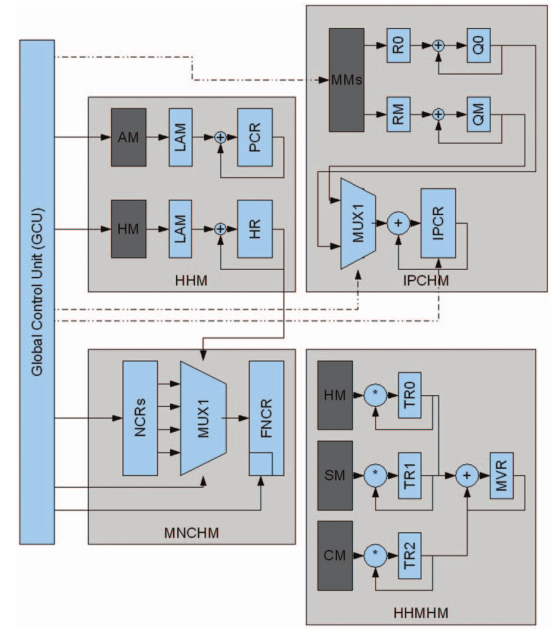
\includegraphics[width=0.9\textwidth]{Figs/2021_Peptidos01}
\end{columns}     
}

\frame{
\frametitle{Resultados}
\begin{columns}
    \column {0.5\textwidth}


\begin{itemize}
\item Cada secuencia de péptidos estaba representada por un punto fijo número y generado por la placa FPGA, eliminando así el sobrecarga debido a la comunicación de datos CPU-FPGA.

\item Los péptidos usados en este estudio estan formados por cadenas de 9 aminoácidos (20 posibles aminoacidos diferentes, 5 bits para su codificación), implicando 45 bits para cada péptido. 

\item Para generar todas las secuencias de péptidos generadas y evaluadas en la tarjeta FPGA se utilizó un contador binario.

	   
\end{itemize}
    
    
    \column {0.5\textwidth} 
\begin{itemize}    
    \item La implementación tiene la misma precisión que la versión de software del mismo.
    \item Individualmente, cada uno de los 4 cálculos de propiedades fisicoquímicas se aceleraron de 17 a 195 veces con la implementación FPGA propuesta.
\end{itemize}
   \begin{center} 
    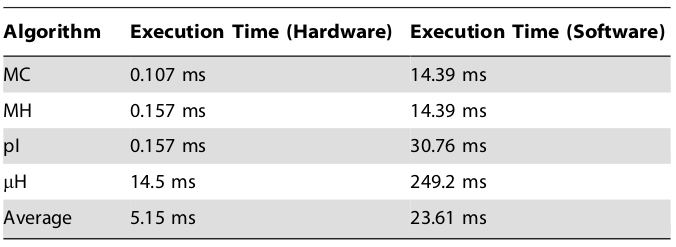
\includegraphics[width=0.9\textwidth]{Figs/2021_Peptidos02}
    \end{center} 
\end{columns}     
}
